%%% Preamble
\documentclass[paper=a4,fontsize=11pt]{report}


\begin{document}

%\begin{titlepage}
    
\newcommand{\HRule}{\rule{\linewidth}{0.5mm}} % Defines a new command for the horizontal lines, change thickness here
    
\center % Center everything on the page
     
%----------------------------------------------------------------------------------------
%	HEADING SECTIONS
%----------------------------------------------------------------------------------------
    
\textsc{\LARGE Instituto Tecnológico de Buenos Aires}\\[2cm] % Name of your university/college
\textsc{\Large Electronica III}\\[1.5cm] % Major heading such as course name
\textsc{\large Trabajo Práctico N° 2}\\[0.5cm] % Minor heading such as course title
    
%----------------------------------------------------------------------------------------
%	TITLE SECTION
%----------------------------------------------------------------------------------------
    
\HRule \\[0.5cm]
{ \huge \bfseries Trabajo Práctico de Laboratorio Nr. 2}\\[0.4cm] % Title of your document
\HRule \\[2cm]
     
%----------------------------------------------------------------------------------------
%	AUTHOR SECTION
%----------------------------------------------------------------------------------------
    
\begin{minipage}{0.4\textwidth}
\begin{flushleft} \large
\emph{Grupo 2:}\\		%names
[.3cm]
Victor \textsc{Oh}\\
Leg. ???\\ 
[.3cm]
Ian \textsc{Diaz}\\
Leg. ???\\ 
[.3cm]
Benjamín Carlos \textsc{Lin}\\
Leg. 57242 \\ 
[.3cm]
Malena \textsc{Muller}\\
Leg. ???\\ 
[.3cm]
\end{flushleft}
\end{minipage}
~
\begin{minipage}{0.4\textwidth}
\begin{flushright} \large
%\emph{Profesor:} \\
%[.3cm]
%Pablo  \textsc{Cossutta}\\ % Supervisor's Name
%Alejandra \textsc{Weill} \\% Supervisor's Name
%Matías  \textsc{Salvati} % Supervisor's Name
\end{flushright}
\end{minipage}\\[2cm]
    
%----------------------------------------------------------------------------------------
%	DATE SECTION
%----------------------------------------------------------------------------------------
    
\vfill
{\large Entregado: 17 de Octubre de 2018}\\[2cm]
    
\vfill 
    
\end{titlepage}
%
%\pagenumbering{roman}
%\tableofcontents
%\newpage
%\pagenumbering{arabic}
%
%Test Text

\section{\color{olive}Exercise 5: Compatibility between TTL and CMOS}

Connecting the following circuit in figure \ref{fig:ej5ttl} and \ref{fig:ej5cmos} leaving one of the inputs floating having $Vcc = 5V$. 

\begin{figure}[h!]
         \begin{minipage}{.47\linewidth}
        \centering
        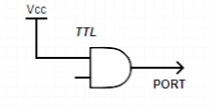
\includegraphics[width=.6\linewidth]{./TTL5.png}
        \caption{\color{cyan}TTL Circuit}
        \label{fig:ej5ttl}
        \end{minipage}
         \begin{minipage}{.5\linewidth}
        \centering
        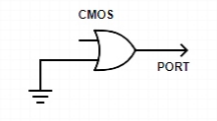
\includegraphics[width=.5\linewidth]{./CMOS5.png}
        \caption{\color{cyan}CMOS Circuit}
        \label{fig:ej5cmos}
    \end{minipage}
\end{figure}

For the 74LS08, the TTL component, the output port value shown was a logical 1 constantly. On the other hand, the 74HC32, the CMOS component, the results were random at a frequency of 50Hz, having variation from being a quadratic function from 0 to 5V, a 

\begin{figure}[h!]
        \centering
        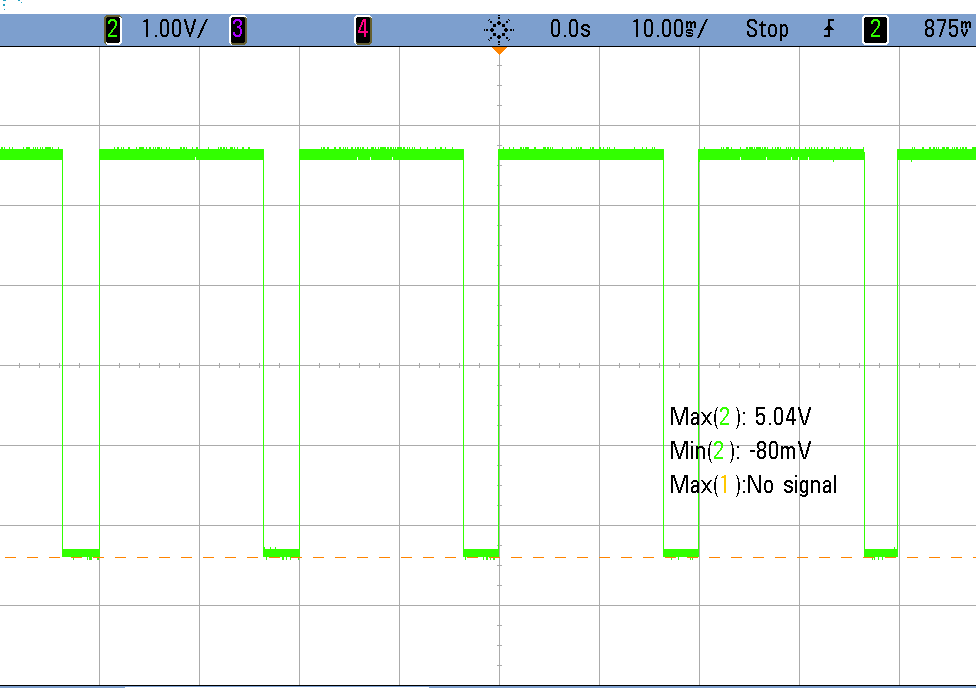
\includegraphics[scale=0.19]{cmos_cerda2.png}\hspace{1cm}
%        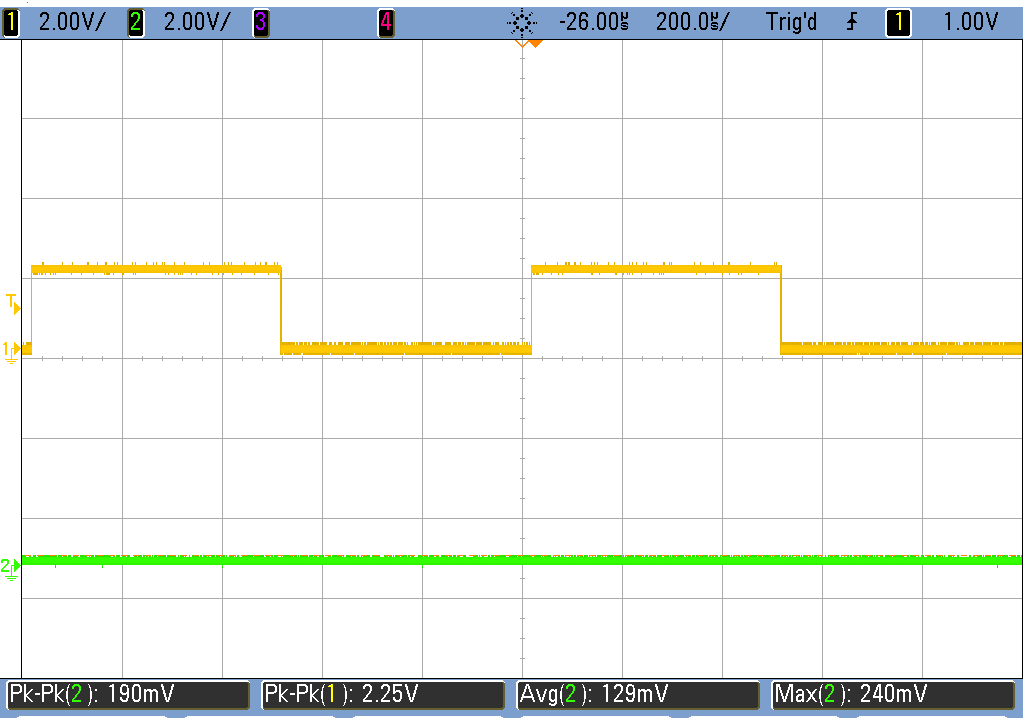
\includegraphics[scale=0.19]{HC-LS-2V.png}\\
        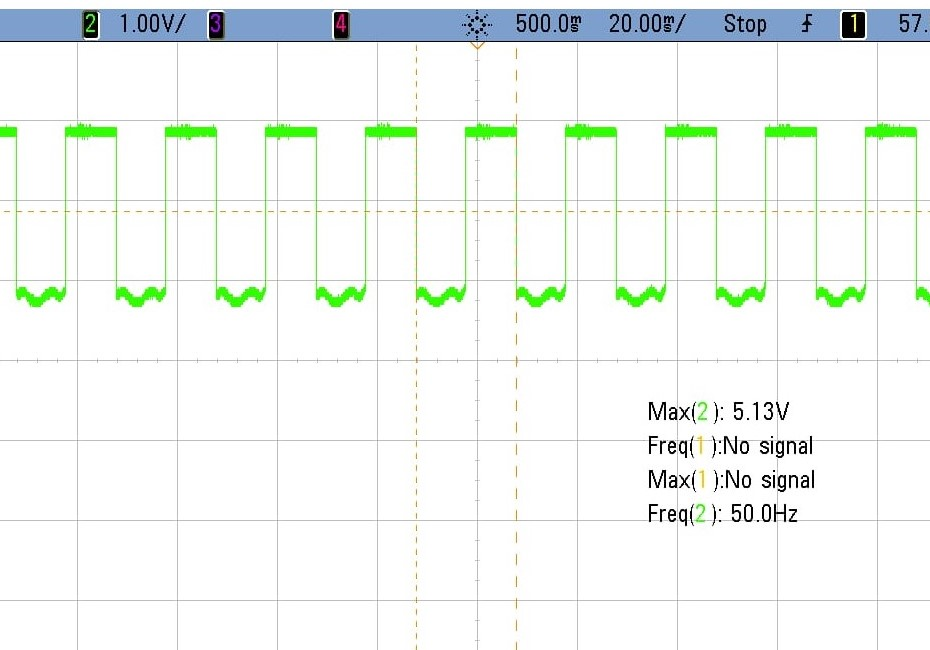
\includegraphics[scale=0.2]{cmos_dads.jpeg}\\
		\vspace{0.2cm}
%		\hspace{0.9cm}
	   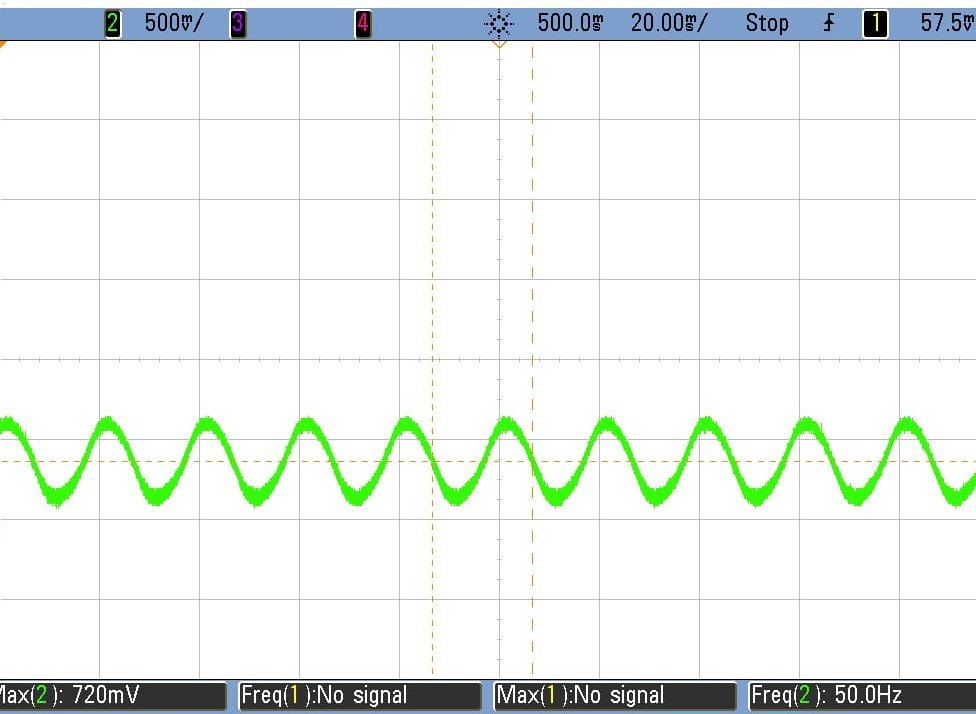
\includegraphics[scale=0.19]{cmos_ahifdas.jpeg} 
%        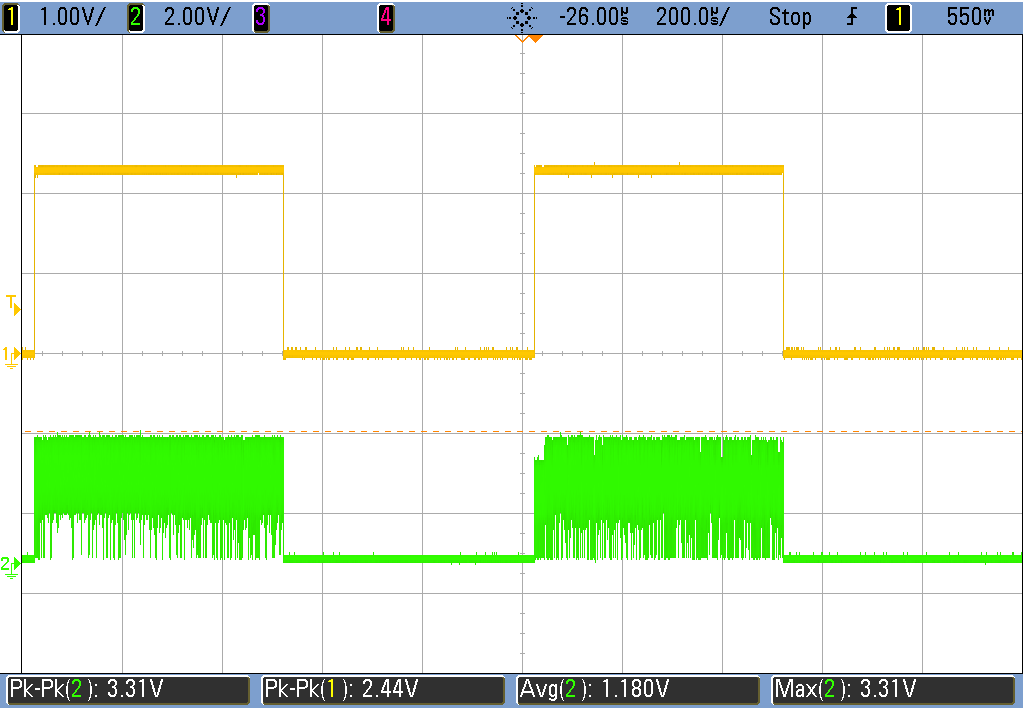
\includegraphics[scale=0.19]{HC-LS-2p3V.png}
        \caption{\color{cyan}74HC02 load to 74LS02}
        \label{fig:ej2exhctols}
    \end{figure}


\end{document}